
\hypertarget{menu_view}{}
\section{View}
\index{view menu}

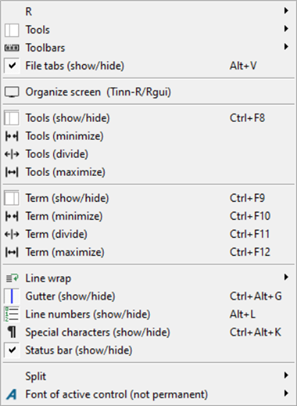
\includegraphics[scale=0.50]{./res/menu_view.png}\\

\begin{scriptsize}
  \begin{tabularx}{\textwidth}{>{\hsize=0.7\hsize}X>{\hsize=0.7\hsize}X}\\
    \hline
    \textbf{Option} & \textbf{Description} \\
    \hline
    R & \textit{\href{\#menu\_view\_r}{See options ...}} \\
    Tools & \textit{\href{\#menu\_view\_tools}{See options ...}} \\
    Toolsbar & \textit{\href{\#menu\_view\_toolbars}{See options ...}} \\
    Tabs & \textit{\href{\#menu\_view\_tabs}{See options ...}} \\
    Organize screen (Tinn-R/Rgui) & Organizes the screen (Tinn-R and Rgui) according to the user set. \textit{\href{\#working\_app\_r}{See options ...}} \\
    Tools (show/hide) & Toggles (show/hide) \textit{Tools} interface \\
    Tools (maximize) & Maximizes the \textit{Tools} interface \\
    Tools (divide) & Divides the \textit{Tools} interface \\
    Tools (minimize) & Minimizes the \textit{Tools} interface \\
    Rterm (show/hide) & Toggles (show/hide) Rterm interface \\
    Rterm (maximize) & Maximizes the Rterm interface \\
    Rterm (divide) & Splits the Rterm interface \\
    Rterm (minimize) & Minimizes the Rterm interface \\
    Line wrap (show/hide) & \textit{\href{\#menu\_view\_linewrap}{See options ...}} \\
    Gutter (show/hide) & Toggles (show/hide) gutter \\
    Line numbers (show/hide) & Toggles (show/hide) line numbers \\
    Special characters (show/hide) & Toggles (show/hide) special characters \\
    Status bar (show/hide) & Toggles (show/hide) status bar \\
    Split & \textit{\href{\#menu\_view\_split}{See options ...}} \\
    Font of active control (not permanent) & \textit{\href{\#menu\_view\_fontsize}{See options ...}} \\
    \hline
  \end{tabularx}
\end{scriptsize}


\hypertarget{menu_view_r}{}
\subsection{R}
\index{view menu!R}

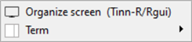
\includegraphics[scale=0.50]{./res/menu_view_r.png}\\

\begin{scriptsize}
  \begin{tabularx}{\textwidth}{>{\hsize=0.5\hsize}X>{\hsize=0.7\hsize}X}\\
    \hline
    \textbf{Option} & \textbf{Description} \\
    \hline
    Organize screen (Tinn-R/Rgui) & Organizes the screen (Tinn-R and Rgui) according to the user set. \textit{\href{\#working\_app\_r}{See options ...}} \\
    Rterm & \textit{\href{\#menu\_view\_r\_rterm}{See options ...}} \\
    \hline
  \end{tabularx}
\end{scriptsize}


\hypertarget{menu_view_r_rterm}{}
\subsubsection{Rterm}\\
\index{view menu!Rterm}

\includegraphics[scale=0.50]{./res/menu_view_r_rterm.png}\\

\begin{scriptsize}
  \begin{tabularx}{\textwidth}{>{\hsize=0.7\hsize}X>{\hsize=0.7\hsize}X}\\
    \hline
    \textbf{Option} & \textbf{Description} \\
    \hline
    Rterm (show/hide) & Toggles (show/hide) Rterm interface \\
    Size & \textit{\href{\#menu\_view\_r\_rterm\_size}{See options ...}} \\
    Split & \textit{\href{\#menu\_view\_r\_rterm\_split}{See options ...}} \\
    Highlighter & \textit{\href{\#menu\_view\_r\_rterm\_highlighter}{See options ...}} \\
    Line wrap & \textit{\href{\#menu\_r\_rterm\_linewrap}{See options ...}} \\
    Font of active control (not permanent) & \textit{\href{\#menu\_r\_rterm\_fontsize}{See options ...}} \\
    \hline
  \end{tabularx}
\end{scriptsize}


\hypertarget{menu_view_r_rterm_size}{}
\subsubsection{Size}\\
\index{view menu!Rterm size}

\includegraphics[scale=0.50]{./res/menu_r_rterm_size.png}\\

\begin{scriptsize}
  \begin{tabularx}{\textwidth}{>{\hsize=0.3\hsize}X>{\hsize=0.7\hsize}X}\\
    \hline
    \textbf{Option} & \textbf{Description} \\
    \hline
    Rterm (maximize) & Maximizes the Rterm interface \\
    Rterm (divide) & Splits the Rterm interface \\
    Rterm (minimize) & Minimizes the Rterm interface \\
    \hline
  \end{tabularx}
\end{scriptsize}


\hypertarget{menu_view_r_rterm_split}{}
\subsubsection{Split}\\
\index{view menu!Rterm split}

\includegraphics[scale=0.50]{./res/menu_r_rterm_split.png}\\

\begin{scriptsize}
  \begin{tabularx}{\textwidth}{>{\hsize=1\hsize}X>{\hsize=0.7\hsize}X}\\
    \hline
    \textbf{Option} & \textbf{Description} \\
    \hline
    Horizontal split (IO and LOG in the same view) & Horizontally splits the Rterm interface placing \textit{IO} and \textit{LOG} in the same view \\
    Vertical split (IO and LOG in the same view) & Vertically splits the Rterm interface placing \textit{IO} and \textit{LOG} in the same view \\
    Remove split (IO and LOG in distinct view) & Removes split placing \textit{IO} and \textit{LOG} in distinct view \\
    \hline
  \end{tabularx}
\end{scriptsize}


\newpage
\hypertarget{menu_view_r_rterm_highlighter}{}
\subsubsection{Highlighter}\\
\index{view menu!Rterm highlighter}

\includegraphics[scale=0.50]{./res/menu_r_rterm_highlighter.png}\\

\begin{scriptsize}
  \begin{tabularx}{\textwidth}{>{\hsize=0.3\hsize}X>{\hsize=0.7\hsize}X}\\
    \hline
    \textbf{Option} & \textbf{Description} \\
    \hline
    IO & \textit{\href{\#menu\_r\_rterm\_highlighter\_IO}{See options ...}} \\
    LOG & \textit{\href{\#menu\_r\_rterm\_highlighter\_Log}{See options ...}} \\
    \hline
  \end{tabularx}
\end{scriptsize}


\hypertarget{menu_view_r_rterm_highlighter_IO}{}
\subsubsection{Highlighter IO}\\
\index{view menu!Rterm highlighter IO}

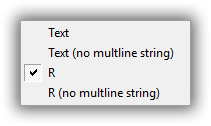
\includegraphics[scale=0.50]{./res/menu_r_rterm_highlighter_io.png}\\

\begin{scriptsize}
  \begin{tabularx}{\textwidth}{>{\hsize=0.3\hsize}X>{\hsize=0.7\hsize}X}\\
    \hline
    \textbf{Option} & \textbf{Description} \\
    \hline
    Text & Sets the IO highlighter to Text \\
    Text (no multline string) & Sets the IO highlighter to Text without string multline suport \\
    R & Sets the IO highlighter to R \\
    R (no multline string) & Sets the IO highlighter to R without string multline suport \\
    \hline
  \end{tabularx}
\end{scriptsize}


\hypertarget{menu_view_r_rterm_highlighter_Log}{}
\subsubsection{Highlighter LOG}\\
\index{view menu!Rterm highlighter LOG}

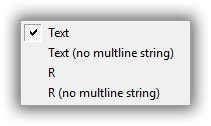
\includegraphics[scale=0.50]{./res/menu_r_rterm_highlighter_log.png}\\

\begin{scriptsize}
  \begin{tabularx}{\textwidth}{>{\hsize=0.3\hsize}X>{\hsize=0.7\hsize}X}\\
    \hline
    \textbf{Option} & \textbf{Description} \\
    \hline
    Text & Sets the LOG highlighter to Text \\
    Text (no multline string) & Sets the LOG highlighter to Text without string multline suport \\
    R & Sets the LOG highlighter to R \\
    R (no multline string) & Sets the LOG highlighter to R without string multline suport \\
    \hline
  \end{tabularx}
\end{scriptsize}


\hypertarget{menu_view_r_rterm_linewrap}{}
\subsubsection{Line wrap}\\
\index{view menu!Rterm line wrap}

\includegraphics[scale=0.50]{./res/menu_r_rterm_linewrap.png}\\

\begin{scriptsize}
  \begin{tabularx}{\textwidth}{>{\hsize=0.3\hsize}X>{\hsize=0.7\hsize}X}\\
    \hline
    \textbf{Option} & \textbf{Description} \\
    \hline
    IO & Sets Line wrap to IO \\
    LOG & Sets Line wrap to LOG \\
    \hline
  \end{tabularx}
\end{scriptsize}


\hypertarget{menu_r_rterm_fontsize}{}
\subsubsection{Font of active control (not permanent)}\\

\includegraphics[scale=0.50]{./res/menu_fontsize_generic.png}\\

\begin{scriptsize}
  \begin{tabularx}{\textwidth}{>{\hsize=0.3\hsize}X>{\hsize=0.7\hsize}X}\\
    \hline
    \textbf{Option} & \textbf{Description} \\
    \hline
    Increase & Increase font size \\
    Decrease & Decrease font size \\
    \hline
  \end{tabularx}
\end{scriptsize}


\hypertarget{menu_view_tools}{}
\subsection{Tools}
\index{view menu!tools}

\includegraphics[scale=0.50]{./res/menu_view_tools.png}\\

\begin{scriptsize}
  \begin{tabularx}{\textwidth}{>{\hsize=0.3\hsize}X>{\hsize=0.7\hsize}X}\\
    \hline
    \textbf{Option} & \textbf{Description} \\
    \hline
    Tools (show/hide) & Toggles (show/hide) \textit{Tools} interface \\
    Size & \textit{\href{\#menu\_view\_tools\_size}{See options ...}} \\
    Resources & \textit{\href{\#menu\_view\_tools\_resources}{See options ...}} \\
    \hline
  \end{tabularx}
\end{scriptsize}


\hypertarget{menu_view_tools_size}{}
\subsubsection{Size}\\
\index{view menu!tools size}

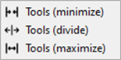
\includegraphics[scale=0.50]{./res/menu_view_tools_size.png}\\

\begin{scriptsize}
  \begin{tabularx}{\textwidth}{>{\hsize=0.3\hsize}X>{\hsize=0.7\hsize}X}\\
    \hline
    \textbf{Option} & \textbf{Description} \\
    \hline
    Tools (maximize) & Maximizes the \textit{Tools} interface \\
    Tools (divide) & Divides the \textit{Tools} interface \\
    Tools (minimize) & Minimizes the \textit{Tools} interface \\
    \hline
  \end{tabularx}
\end{scriptsize}


\hypertarget{menu_view_tools_resources}{}
\subsubsection{Resources}\\
\index{view menu!tools resources}

\includegraphics[scale=0.50]{./res/menu_view_tools_resources.png}\\

\begin{scriptsize}
  \begin{tabularx}{\textwidth}{>{\hsize=0.4\hsize}X>{\hsize=0.7\hsize}X}\\
    \hline
    \textbf{Option} & \textbf{Description} \\
    \hline
    Misc & \textit{\href{\#menu\_view\_tools\_resources\_misc}{See options ...}} \\
    Markup & \textit{\href{\#menu\_view\_tools\_resources\_markup}{See options ...}} \\
    Results & \textit{\href{\#menu\_view\_tools\_resources\_results}{See options ...}} \\
    Shortcuts (show/hide) & Toggles (show/hide) \textit{Shortcuts} tab of \textit{Tools} interface \\
    Spell (show/hide) & Toggles (show/hide) \textit{Spell} tab of \textit{Tools} interface \\
    Database & \textit{\href{\#menu\_view\_tools\_resources\_database}{See options ...}} \\
    R & \textit{\href{\#menu\_view\_tools\_resources\_r}{See options ...}} \\
    \hline
  \end{tabularx}
\end{scriptsize}


\newpage
\hypertarget{menu_view_tools_resources_misc}{}
\subsubsection{Misc}\\
\index{view menu!tools resources misc}

\includegraphics[scale=0.50]{./res/menu_view_tools_resources_misc.png}\\

\begin{scriptsize}
  \begin{tabularx}{\textwidth}{>{\hsize=0.5\hsize}X>{\hsize=0.7\hsize}X}\\
    \hline
    \textbf{Option} & \textbf{Description} \\
    \hline
    Misc (show/hide) & Toggles (show/hide) \textit{Misc} tab of \textit{Tools} interface \\
    Windows expl. (show/hide) & Toggles (show/hide) \textit{Windows expl.} tab of \textit{Misc} \\
    Work expl. (show/hide) & Toggles (show/hide) \textit{Work expl.} tab of \textit{Misc} \\
    Project (show/hide) & Toggles (show/hide) \textit{Project} tab of \textit{Misc} \\
    \hline
  \end{tabularx}
\end{scriptsize}


\hypertarget{menu_view_tools_resources_markup}{}
\subsubsection{Markup}\\
\index{view menu!tools resources markup}

\includegraphics[scale=0.50]{./res/menu_view_tools_resources_markup.png}\\

\begin{scriptsize}
  \begin{tabularx}{\textwidth}{>{\hsize=0.3\hsize}X>{\hsize=0.7\hsize}X}\\
    \hline
    \textbf{Option} & \textbf{Description} \\
    \hline
    Markup (show/hide) & Toggles (show/hide) \textit{Markup} tab of \textit{Tools} interface \\
    Txt2tags (show/hide) & Toggles (show/hide) \textit{Txt2tags} tab of \textit{Markup} \\
    \LaTeX ~(show/hide) & Toggles (show/hide) \LaTeX ~tab of \textit{Markup} \\
    \hline
  \end{tabularx}
\end{scriptsize}


\hypertarget{menu_view_tools_resources_results}{}
\subsubsection{Results}\\
\index{view menu!tools resources results}

\includegraphics[scale=0.50]{./res/menu_view_tools_resources_results.png}\\

\begin{scriptsize}
  \begin{tabularx}{\textwidth}{>{\hsize=0.3\hsize}X>{\hsize=0.7\hsize}X}\\
    \hline
    \textbf{Option} & \textbf{Description} \\
    \hline
    Results (show/hide) & Toggles (show/hide) \textit{Results} tab of \textit{Tools} interface \\
    Ini lOG (show/hide) & Toggles (show/hide) \textit{Ini lOG} tab of \textit{Results} \\
    Search (show/hide) & Toggles (show/hide) \textit{Search} tab of \textit{Results} \\
    \hline
  \end{tabularx}
\end{scriptsize}


\hypertarget{menu_view_tools_resources_database}{}
\subsubsection{Database}\\
\index{view menu!tools resources database}

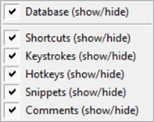
\includegraphics[scale=0.50]{./res/menu_view_tools_resources_database.png}\\

\begin{scriptsize}
  \begin{tabularx}{\textwidth}{>{\hsize=0.3\hsize}X>{\hsize=0.7\hsize}X}\\
    \hline
    \textbf{Option} & \textbf{Description} \\
    \hline
    Database (show/hide) & Toggles (show/hide) \textit{Database} tab of \textit{Tools} interface \\
    Shortcuts (show/hide) & Toggles (show/hide) \textit{Shortcuts} tab of \textit{Database} \\
    Completion (show/hide) & Toggles (show/hide) \textit{Completion} tab of \textit{Database} \\
    Comments (show/hide) & Toggles (show/hide) \textit{Comments} tab of \textit{Database} \\
    \hline
  \end{tabularx}
\end{scriptsize}


\hypertarget{menu_view_tools_resources_r}{}
\subsubsection{R}\\
\index{view menu!tools resources R}

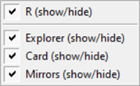
\includegraphics[scale=0.50]{./res/menu_view_tools_resources_r.png}\\

\begin{scriptsize}
  \begin{tabularx}{\textwidth}{>{\hsize=0.3\hsize}X>{\hsize=0.7\hsize}X}\\
    \hline
    \textbf{Option} & \textbf{Description} \\
    \hline
    R (show/hide) & Toggles (show/hide) \textit{R} tab of \textit{Tools} interface \\
    Explorer (show/hide) & Toggles (show/hide) \textit{Explorer} tab of \textit{R} \\
    Card (show/hide) & Toggles (show/hide) \textit{Rcard} tab of \textit{Database} \\
    Mirrors (show/hide) & Toggles (show/hide) \textit{R mirrors} tab of \textit{Database} \\
    \hline
  \end{tabularx}
\end{scriptsize}


\hypertarget{menu_view_toolbars}{}
\subsection{Toolbars}
\index{view menu!toolbars}

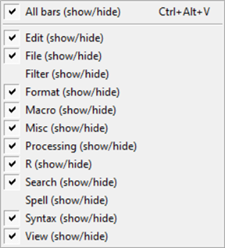
\includegraphics[scale=0.50]{./res/menu_view_toolsbar.png}\\

\begin{scriptsize}
  \begin{tabularx}{\textwidth}{>{\hsize=0.3\hsize}X>{\hsize=0.7\hsize}X}\\
    \hline
    \textbf{Option} & \textbf{Description} \\
    \hline
    All bars (show/hide) & Toggles (show/hide) \textit{All bars} tab of \textit{Tools bar} interface \\
    Edit (show/hide) & Toggles (show/hide) \textit{Edit} tab of \textit{Tools bar} interface \\
    File (show/hide) & Toggles (show/hide) \textit{File} tab of \textit{Tools bar} interface \\
    Filter (show/hide) & Toggles (show/hide) \textit{Filter} tab of \textit{Tools bar} interface \\
    Format (show/hide) & Toggles (show/hide) \textit{Format} tab of \textit{Tools bar} interface \\
    Macro (show/hide) & Toggles (show/hide) \textit{Macro} tab of \textit{Tools bar} interface \\
    Misc (show/hide) & Toggles (show/hide) \textit{Misc} tab of \textit{Tools bar} interface \\
    Processing (show/hide) & Toggles (show/hide) \textit{Processing} tab of \textit{Tools bar} interface \\
    R (show/hide) & Toggles (show/hide) \textit{R} tab of \textit{Tools bar} interface \\
    Search (show/hide) & Toggles (show/hide) \textit{Search} tab of \textit{Tools bar} interface \\
    Spell (show/hide) & Toggles (show/hide) \textit{Spell} tab of \textit{Tools bar} interface \\
    Syntax (show/hide) & Toggles (show/hide) \textit{Syntax} tab of \textit{Tools bar} interface \\
    View (show/hide) & Toggles (show/hide) \textit{View} tab of \textit{Tools bar} interface \\
    \hline
  \end{tabularx}
\end{scriptsize}


\hypertarget{menu_view_tabs}{}
\subsection{Tabs}
\index{view menu!tabs}

\includegraphics[scale=0.50]{./res/menu_view_tabs.png}\\

\begin{scriptsize}
  \begin{tabularx}{\textwidth}{>{\hsize=0.3\hsize}X>{\hsize=0.7\hsize}X}\\
    \hline
    \textbf{Option} & \textbf{Description} \\
    \hline
    Files & \textit{\href{\#menu\_view\_tabs\_files}{See options ...}} \\
    Tools & \textit{\href{\#menu\_view\_tabs\_tools}{See options ...}} \\
    Rterm & \textit{\href{\#menu\_view\_tabs\_rterm}{See options ...}} \\
    \hline
  \end{tabularx}
\end{scriptsize}


\hypertarget{menu_view_tabs_files}{}
\subsubsection{Files}
\index{view menu!tabs files}

\includegraphics[scale=0.50]{./res/menu_view_tabs_files.png}\\

\begin{scriptsize}
  \begin{tabularx}{\textwidth}{>{\hsize=0.3\hsize}X>{\hsize=0.7\hsize}X}\\
    \hline
    \textbf{Option} & \textbf{Description} \\
    \hline
    Tabs (show/hide) & Toogles(show/hide) the main \textit{Tabs} \\
    Top & Shows the main \textit{Tabs} on top \\
    Bottom & Shows the main \textit{Tabs} on bottom \\
    \hline
  \end{tabularx}
\end{scriptsize}


\hypertarget{menu_view_tabs_tools}{}
\subsubsection{Tools}
\index{view menu!tabs tools}

\includegraphics[scale=0.50]{./res/menu_view_tabs_tools.png}\\

\begin{scriptsize}
  \begin{tabularx}{\textwidth}{>{\hsize=0.3\hsize}X>{\hsize=0.7\hsize}X}\\
    \hline
    \textbf{Option} & \textbf{Description} \\
    \hline
    Left & Shows the \textit{Tools Tabs} on left \\
    Top & Shows the \textit{Tools Tabs} on top \\
    Right & Shows the \textit{Tools Tabs} on right \\
    Bottom & Shows the \textit{Tools Tabs} on bottom \\
    \hline
  \end{tabularx}
\end{scriptsize}


\hypertarget{menu_view_tabs_rterm}{}
\subsubsection{Rterm}
\index{view menu!tabs Rterm}

\includegraphics[scale=0.50]{./res/menu_view_tabs_rterm.png}\\

\begin{scriptsize}
  \begin{tabularx}{\textwidth}{>{\hsize=0.3\hsize}X>{\hsize=0.7\hsize}X}\\
    \hline
    \textbf{Option} & \textbf{Description} \\
    \hline
    Left & Shows the \textit{Rterm Tabs} on left \\
    Top & Shows the \textit{Rterm Tabs} on top \\
    Right & Shows the \textit{Rterm Tabs} on right \\
    Bottom & Shows the \textit{Rterm Tabs} on bottom \\
    \hline
  \end{tabularx}
\end{scriptsize}


\hypertarget{menu_view_linewrap}{}
\subsection{Line wrap}
\index{view menu! Line wrap}

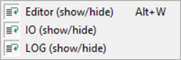
\includegraphics[scale=0.50]{./res/menu_view_linewrap.png}\\

\begin{scriptsize}
  \begin{tabularx}{\textwidth}{>{\hsize=0.3\hsize}X>{\hsize=0.7\hsize}X}\\
    \hline
    \textbf{Option} & \textbf{Description} \\
    \hline
    Editor (show/hide) & Toggles (show/hide) \textit{Editor} line wrap \\
    Rterm/IO (show/hide) & Toggles (show/hide) \textit{Rterm/IO} line wrap \\
    Rterm/LOG (show/hide) & Toggles (show/hide) \textit{Rterm/LOG} line wrap \\
    \hline
  \end{tabularx}
\end{scriptsize}


\hypertarget{menu_view_split}{}
\subsection{Split}
\index{view menu!split}

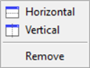
\includegraphics[scale=0.50]{./res/menu_view_split.png}\\

\begin{scriptsize}
  \begin{tabularx}{\textwidth}{>{\hsize=0.3\hsize}X>{\hsize=0.7\hsize}X}\\
    \hline
    \textbf{Option} & \textbf{Description} \\
    \hline
    Horizontal & Horizontally splits the editor \\
    Vertical & Vertically splits the editor \\
    Remove & Removes split \\
    \hline
  \end{tabularx}
\end{scriptsize}


\hypertarget{menu_view_fontsize}{}
\subsection{Font of active control (not permanent)}
\index{view menu!fontsize}

\includegraphics[scale=0.50]{./res/menu_fontsize_generic.png}\\

\begin{scriptsize}
  \begin{tabularx}{\textwidth}{>{\hsize=0.3\hsize}X>{\hsize=0.7\hsize}X}\\
    \hline
    \textbf{Option} & \textbf{Description} \\
    \hline
    Increase & Increase font size \\
    Decrease & Decrease font size \\
    \hline
  \end{tabularx}
\end{scriptsize}
